\documentclass[12pt,a4paper]{article}

% This report follows the exact preamble and cover formatting of reference.tex.
\usepackage[utf8]{inputenc}
\usepackage[T1]{fontenc}
\usepackage{geometry}
\usepackage{listings}
\usepackage{amsmath,amssymb}
\usepackage{graphicx}
\usepackage{booktabs}
\usepackage{array}
\usepackage{enumitem}
\usepackage{hyperref}
\usepackage{float}
\usepackage{eso-pic}

\geometry{left=2.5cm, right=2.5cm, top=2.5cm, bottom=2.5cm}

\lstdefinestyle{plain}{
  basicstyle=\ttfamily\small,
  numberstyle=\tiny,
  numbers=left, numbersep=6pt,
  frame=none,
  breaklines=true, showstringspaces=false,
  tabsize=2, captionpos=b,
  xleftmargin=18pt,
  aboveskip=10pt, belowskip=6pt
}

\setcounter{secnumdepth}{0}
\pagestyle{plain}
\hypersetup{colorlinks=true, linkcolor=black, urlcolor=black}

\begin{document}

% Cover page based on reference.tex.
\thispagestyle{empty}
\AddToShipoutPictureBG{%
  \AtPageLowerLeft{%
    \hspace{1.2cm}\raisebox{1.2cm}{%
      \color{black}\framebox[\dimexpr\paperwidth-2.4cm\relax]{%
        \rule{0pt}{\dimexpr\paperheight-2.4cm\relax}}%
    }%
  }%
}

\begin{center}

\vspace*{1.4cm}

\includegraphics[width=0.22\textwidth]{outputs/emblem.png}\\[0.6cm]

{\Large TRIBHUVAN UNIVERSITY}\\[0.35cm]
{\large INSTITUTE OF ENGINEERING}\\[0.15cm]
{\large PULCHOWK CAMPUS}\\[1.4cm]

{\bfseries\large A LAB REPORT\\
ON\\[0.2cm]
Genetic Algorithm for a Painter Robot}

\vspace{2.2cm}
{\rule{0.3pt}{2.3cm}}\hspace{1.4cm}{\rule{0.3pt}{2.3cm}}\hspace{1.4cm}{\rule{0.3pt}{2.3cm}}

\vspace{2.6cm}
\end{center}

\noindent
\begin{minipage}[t]{0.47\textwidth}
\vspace{0pt}
\underline{\textbf{SUBMITTED BY:}}\\[0.4cm]
Name: Aditya Kumar Shah\\[0.2cm]
Roll No.: 080BCT011\\[0.2cm]
Lab No.: 06
\end{minipage}\hfill
\begin{minipage}[t]{0.47\textwidth}
\vspace{0pt}
\begin{flushright}
\underline{\textbf{SUBMITTED TO:}}\\[0.4cm]
Department of Electronics\\[0.2cm]
and Computer Engineering
\end{flushright}
\end{minipage}

\vfill
\newpage

\section*{1. Objectives}

\begin{enumerate}[leftmargin=1.6em]
  \item To implement a genetic algorithm for a local painter-robot policy.
  \item To evolve 50 random chromosomes of length 54 for 200 generations in a 20 by 40 empty room.
  \item To measure fitness as the average fraction of paintable cells covered from several starting states.
  \item To compare transfer of an empty-room policy with a policy evolved specifically for a furnished room.
\end{enumerate}

\section*{2. Problem Formulation}

The chromosome has one action for each possible local state $[c,f,l,r]$. The current cell $c$ has two values, 0 for unpainted and 2 for painted. The forward, left, and right cells each have three values: 0 for empty, 1 for wall or furniture, and 2 for painted. Therefore,
\[
  2 \times 3 \times 3 \times 3 = 54
\]
possible states are encoded. The gene actions are 0 (no turn), 1 (turn left), 2 (turn right), and 3 (randomly turn left or right).

At every step the painter observes its state, applies its action, paints the current unpainted square, and attempts to move forward. Positions outside the room are treated as walls. A run stops when all paintable cells are covered or when a finite three-pass safety limit is reached.

\section*{3. Assignment 1 --- Hand-designed Strategy}

A suitable strategy for an empty rectangular room is a serpentine or lawn-mower sweep. The painter starts near a corner, moves across one row, turns at the boundary, shifts by one row, and moves across the next row in the opposite direction. This pattern visits nearly every cell once and avoids repeatedly walking through already painted space. The strategy is described conceptually only and is not manually encoded into the chromosome.

\begin{figure}[H]
\centering
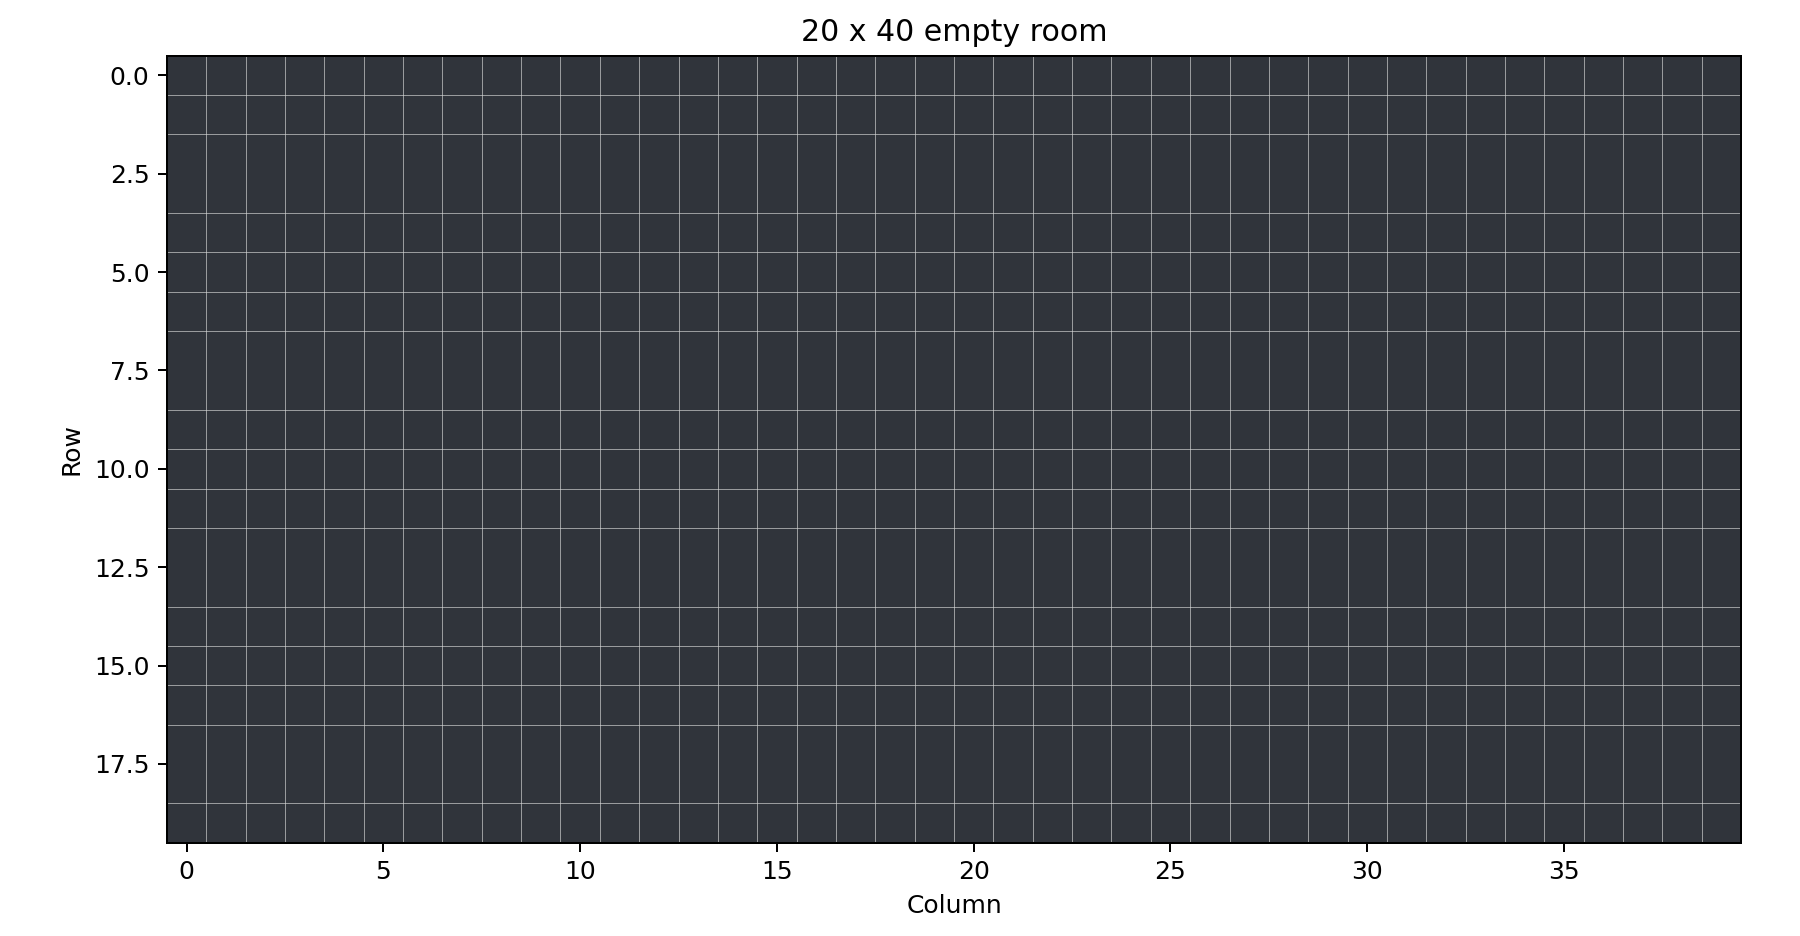
\includegraphics[width=0.46\textwidth]{outputs/empty_room.png}
\hspace{0.04\textwidth}
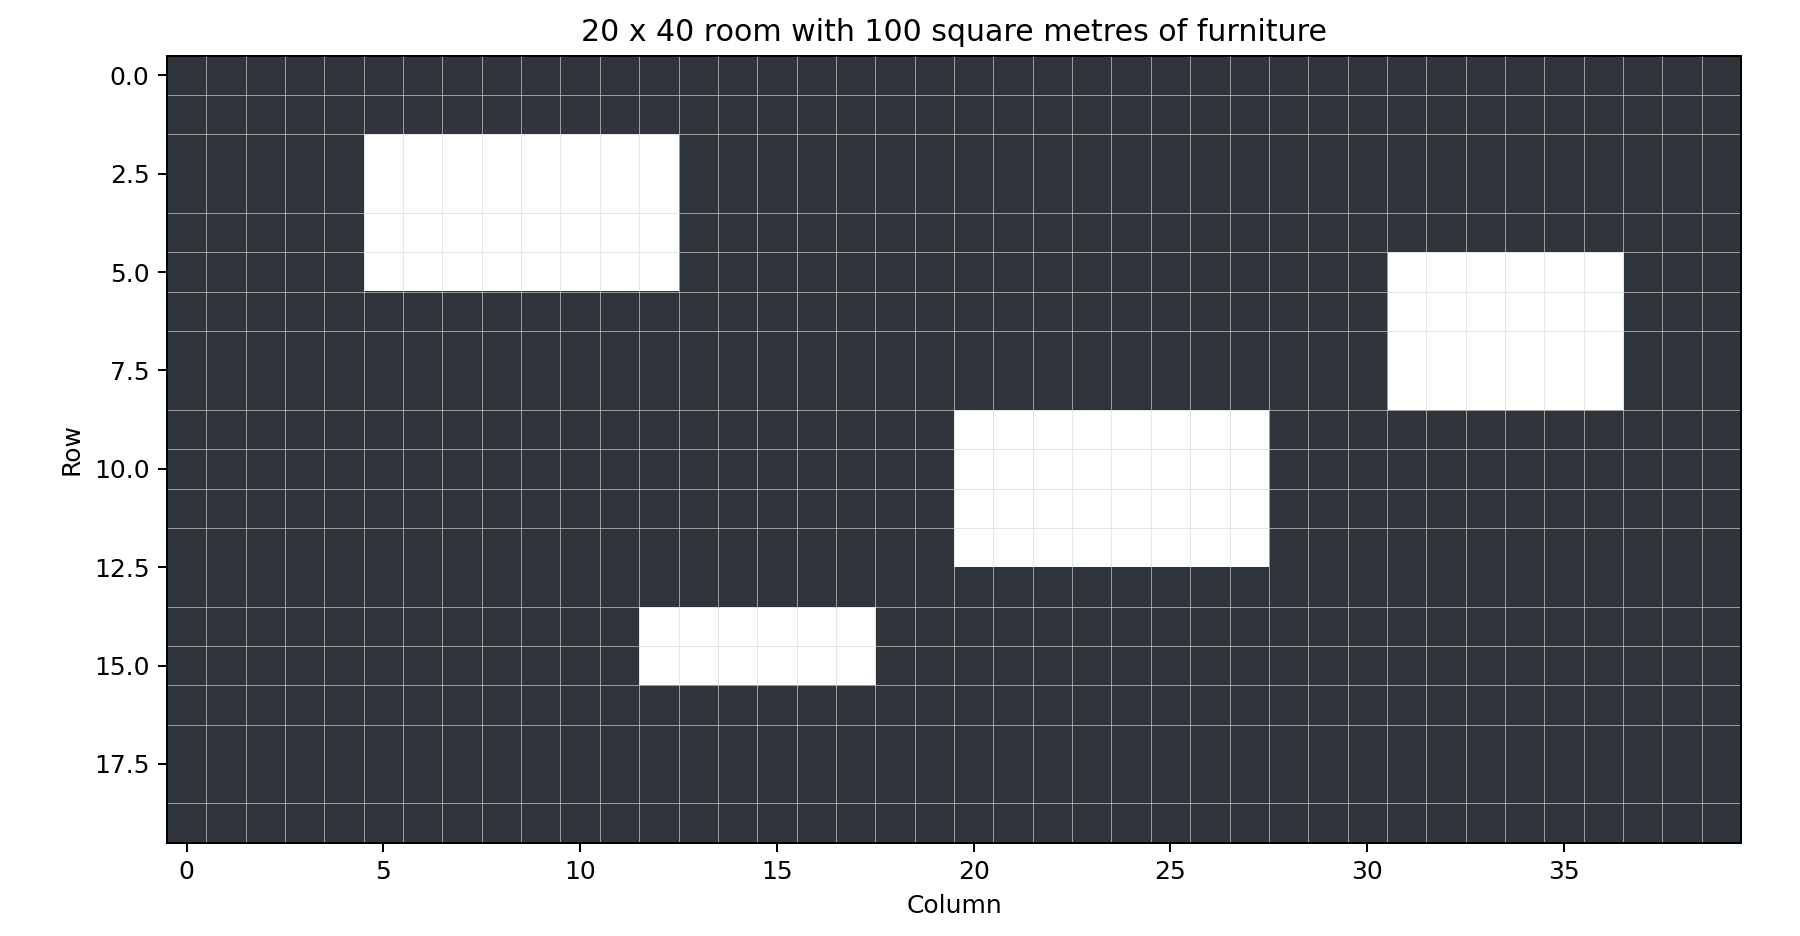
\includegraphics[width=0.46\textwidth]{outputs/furnished_room.png}
\caption{The empty and furnished environments used in the experiments.}
\end{figure}

\section*{4. Genetic Algorithm Design}

The initial population contains 50 chromosomes with uniformly random actions. Fitness is the mean coverage over three fixed training starts. At each generation, two elite chromosomes are copied unchanged. The remaining parents are selected using size-3 tournament selection, followed by single-point crossover and independent mutation with probability 0.002 per locus. The process is repeated for 200 offspring generations.

\begin{center}
\begin{tabular}{@{}ll@{}}
\toprule
\textbf{Parameter} & \textbf{Value} \\
\midrule
Population size & 50 \\
Chromosome length & 54 \\
Generations & 200 \\
Training episodes & 3 per chromosome \\
Validation episodes & 8 \\
Mutation rate & 0.002 per locus \\
Selection & Tournament, size 3, with 2 elites \\
Crossover & Single point \\
\bottomrule
\end{tabular}
\end{center}

\section*{5. Assignment 2 --- Empty-room Experiment}

The 20 by 40 empty room has 800 paintable cells. The population learns a high-coverage policy rapidly. The best validation run covers all 800 cells, and the champion averages 99.08\% across eight validation starts.

\begin{center}
\begin{tabular}{@{}lr@{}}
\toprule
\textbf{Measure} & \textbf{Result} \\
\midrule
Paintable cells & 800 \\
Mean validation efficiency & 99.08\% \\
Best validation efficiency & 100.00\% \\
Worst validation efficiency & 94.12\% \\
Mean steps & 2286.75 \\
\bottomrule
\end{tabular}
\end{center}

\begin{figure}[H]
\centering

\includegraphics[width=0.92\textwidth]{outputs/empty_fitness.png}
\caption{Average, median, and best fitness over generations in the empty room.}
\end{figure}

\begin{figure}[H]
\centering
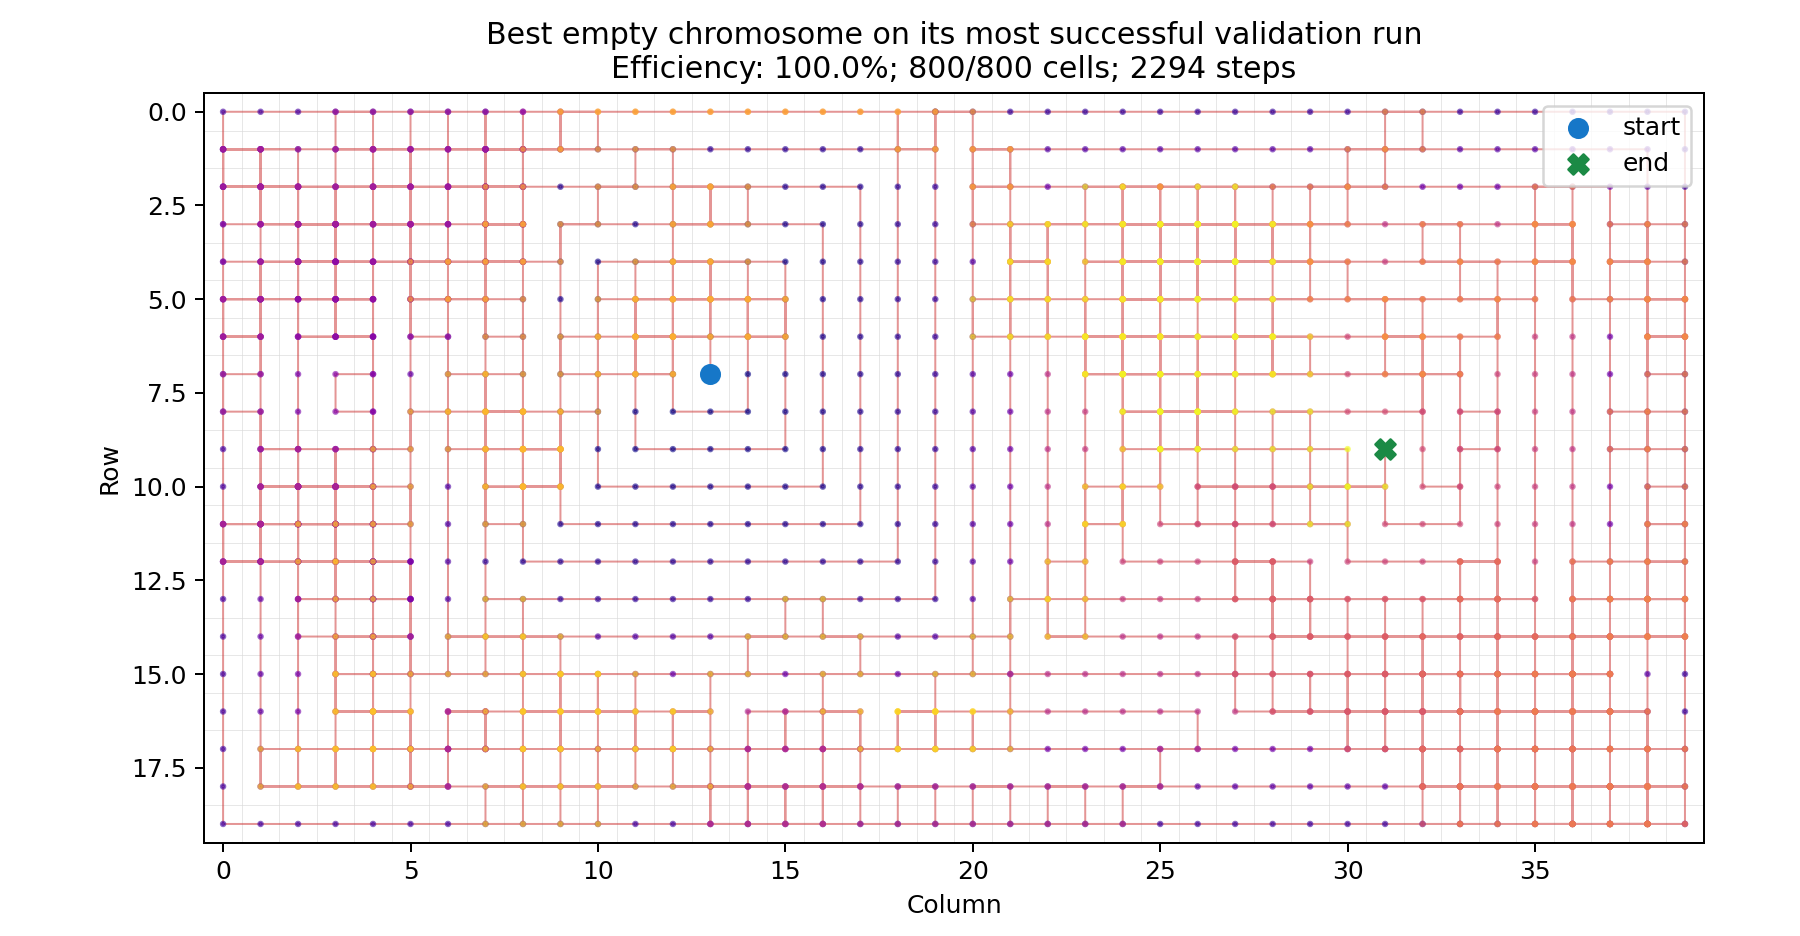
\includegraphics[width=0.92\textwidth]{outputs/empty_best_trajectory.png}
\caption{Trajectory of the empty-room champion on its most successful validation run.}
\end{figure}

\section*{6. Final Population}

The final population shows strong vertical bands at several loci, indicating that selection has made certain actions common for particular local states. Some genes remain variable because different local policies can achieve similar coverage. The complete chromosome values are stored in \texttt{outputs/summary.json}.

\begin{figure}[H]
\centering
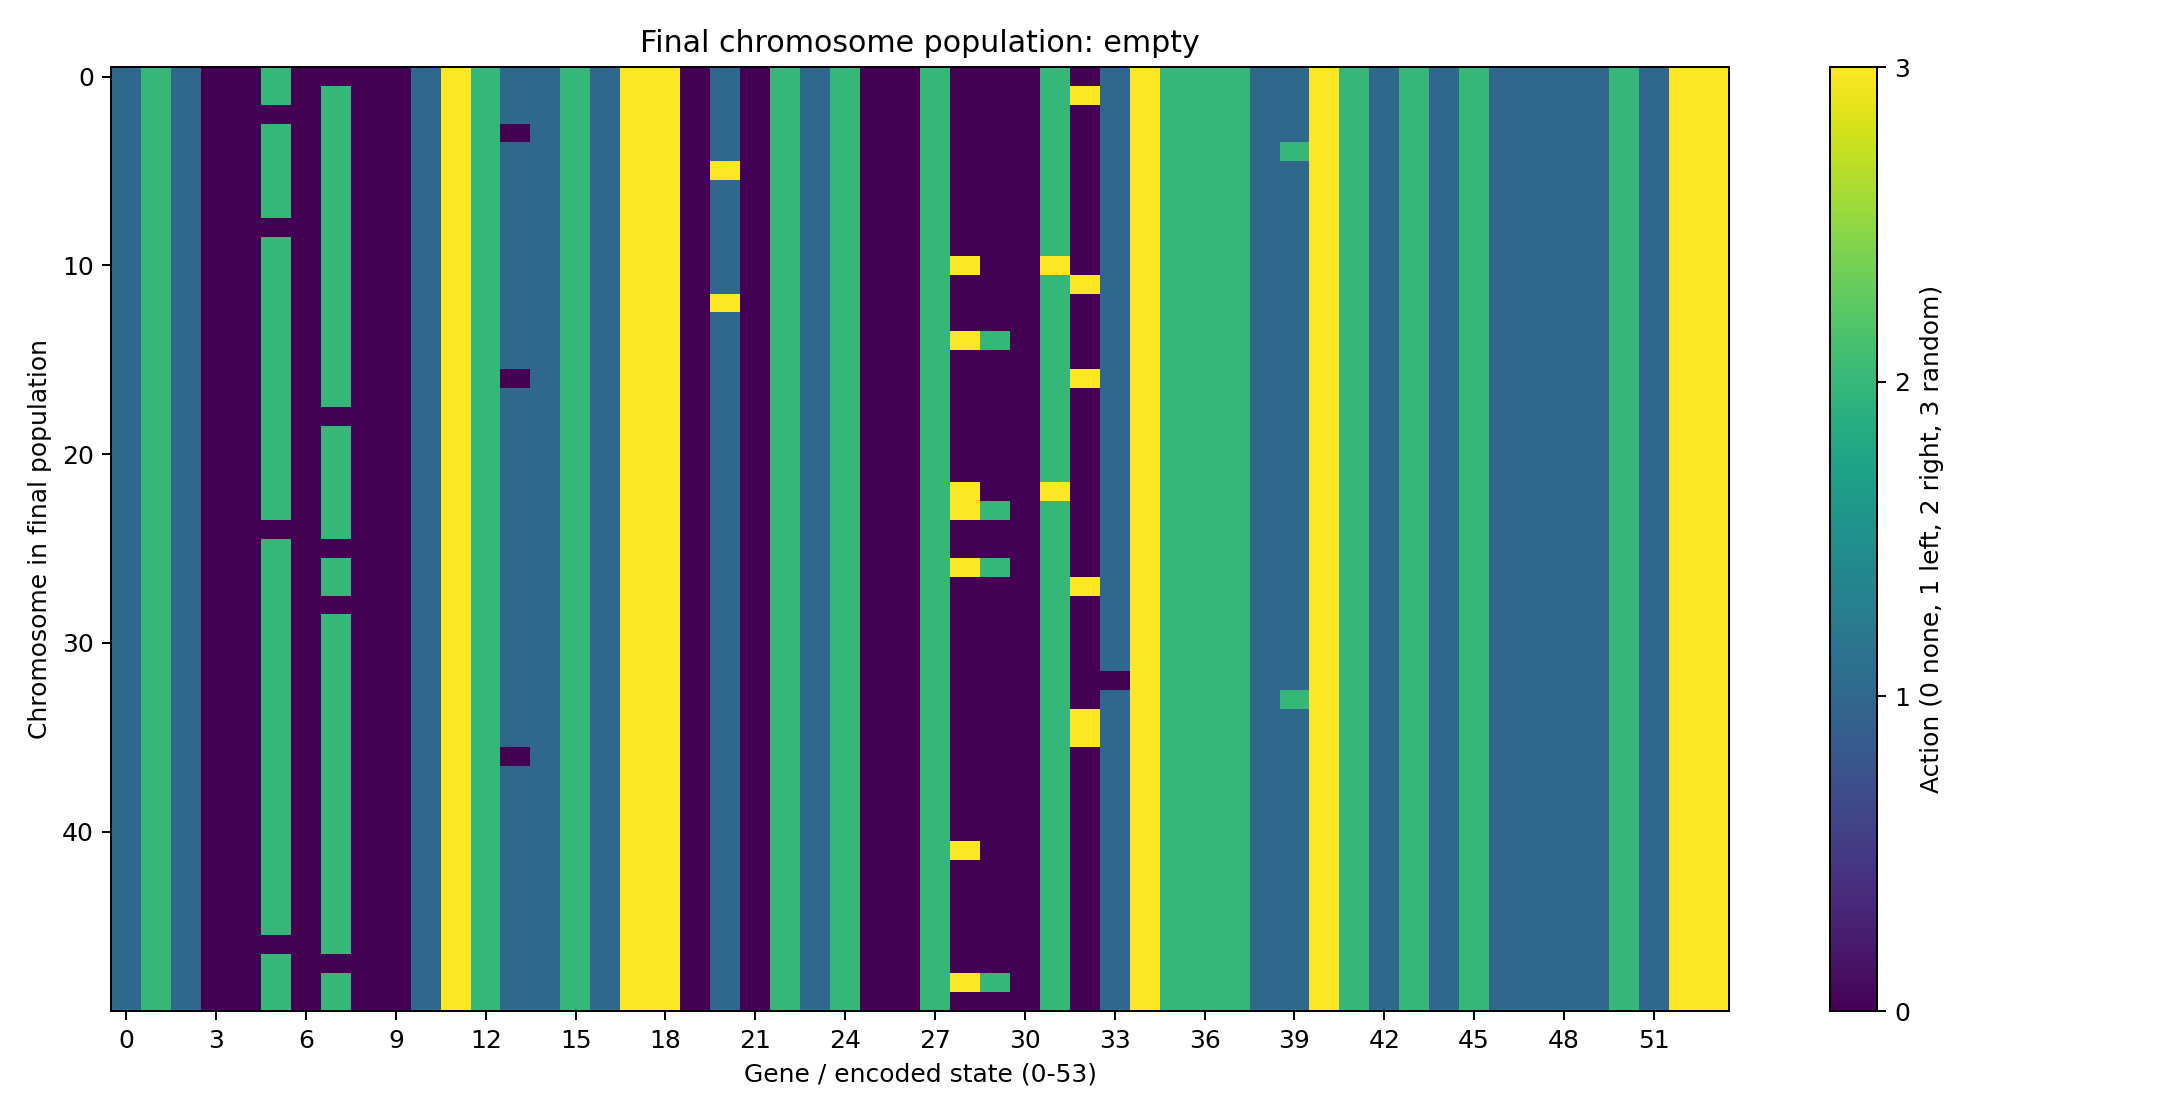
\includegraphics[width=0.92\textwidth]{outputs/empty_final_population.png}
\caption{Final population of 50 chromosomes for the empty-room experiment.}
\end{figure}

\section*{7. Assignment 3 --- Strategic Innovations}

Two possible innovations that increase fitness are:

\begin{enumerate}[leftmargin=1.6em]
  \item A rule that turns when the forward cell is blocked and follows the open side of a wall instead of repeatedly attempting the same move.
  \item A combination of rules that uses painted neighbours as a local cue: it continues along an unpainted strip and turns at a painted boundary to enter another strip, approximating the serpentine sweep without global memory.
\end{enumerate}

The large early jumps in the fitness curves occur when a chromosome first combines enough such behaviours to reduce repeated movement and reach previously missed regions.

\section*{8. Assignment 4 --- Furniture and Transfer}

The furnished room contains four rectangular obstacles with a total area of 100 square metres, leaving 700 paintable cells. When the empty-room champion is transferred without modification, the obstacles interrupt its learned straight sweeps. Depending on the start position, it can repeat corridors, turn around the wrong side of an obstacle, or leave pockets of unpainted space near furniture.

\begin{center}
\small
\begin{tabular}{@{}lrrrr@{}}
\toprule
\textbf{Experiment} & \textbf{Mean} & \textbf{Best} & \textbf{Worst} & \textbf{Cells} \\
\midrule
Empty champion on furnished room & 94.61\% & 99.57\% & 82.14\% & 700 \\
Fresh GA on furnished room & 98.89\% & 99.57\% & 97.29\% & 700 \\
\bottomrule
\end{tabular}
\end{center}

On a stricter paired test using the same eight furnished-room starts, the transferred empty-room champion averaged 80.88\%, including one run at 0.14\%, while the furnished-room champion averaged 98.89\%. This demonstrates that the furniture-specific policy is more robust to starting position.

\begin{figure}[H]
\centering
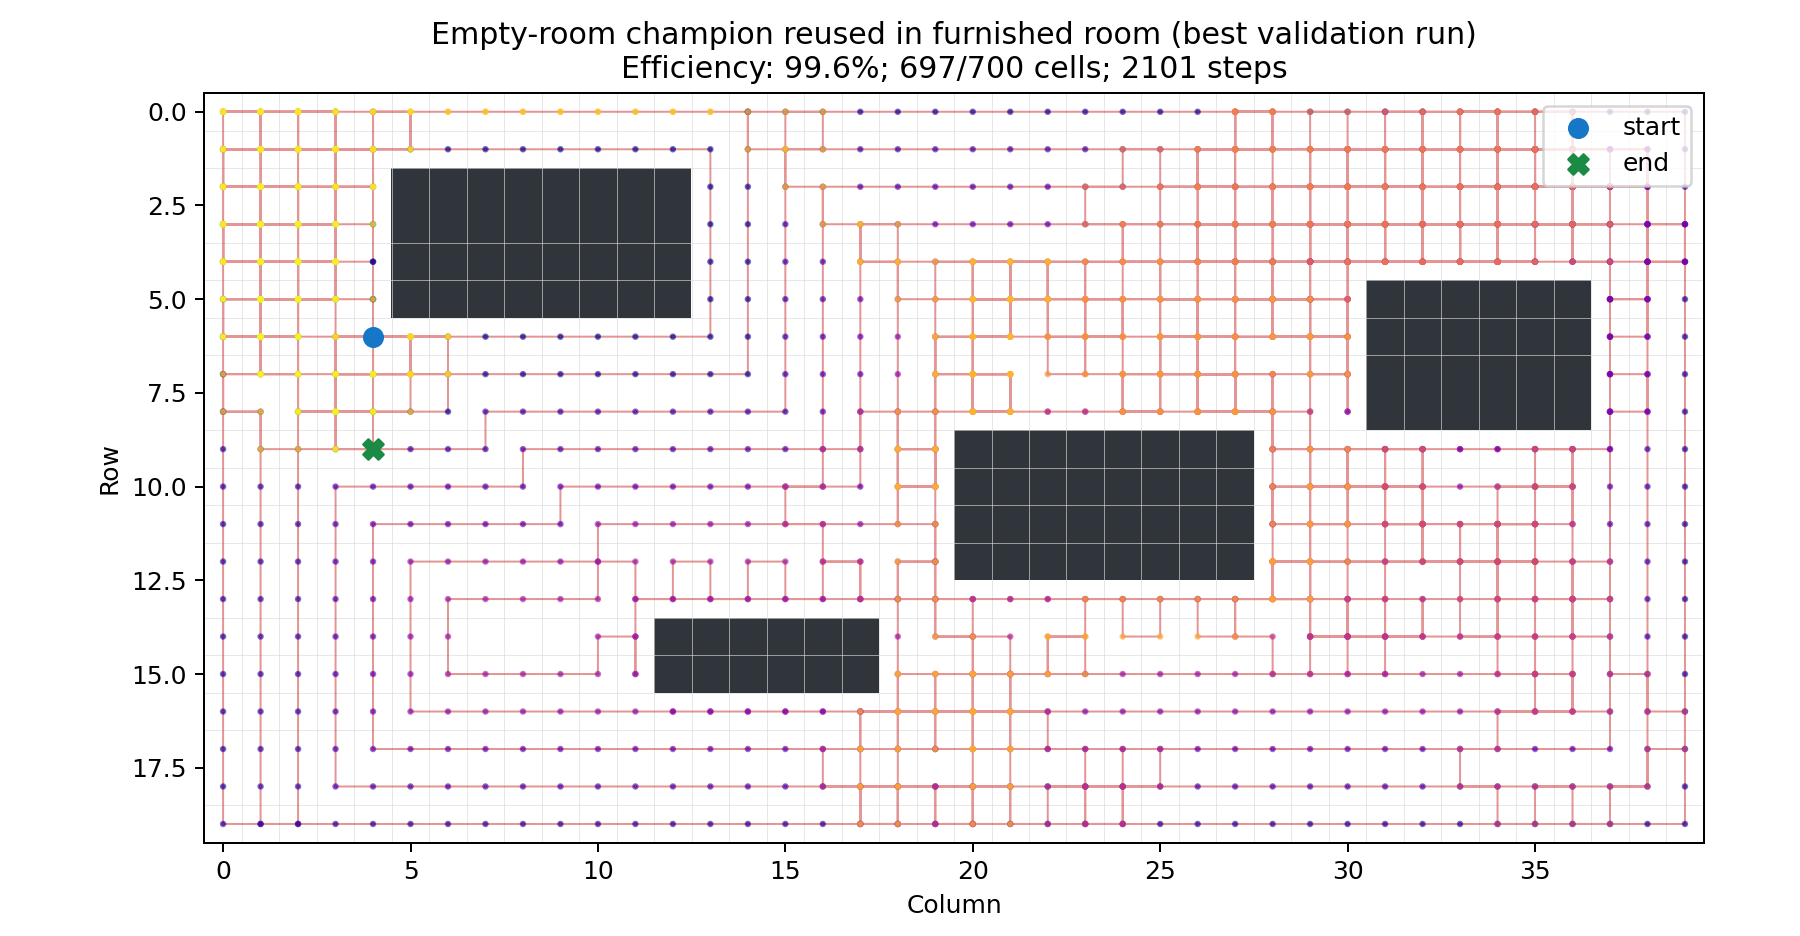
\includegraphics[width=0.46\textwidth]{outputs/furnished_reuse_trajectory.png}
\hspace{0.04\textwidth}
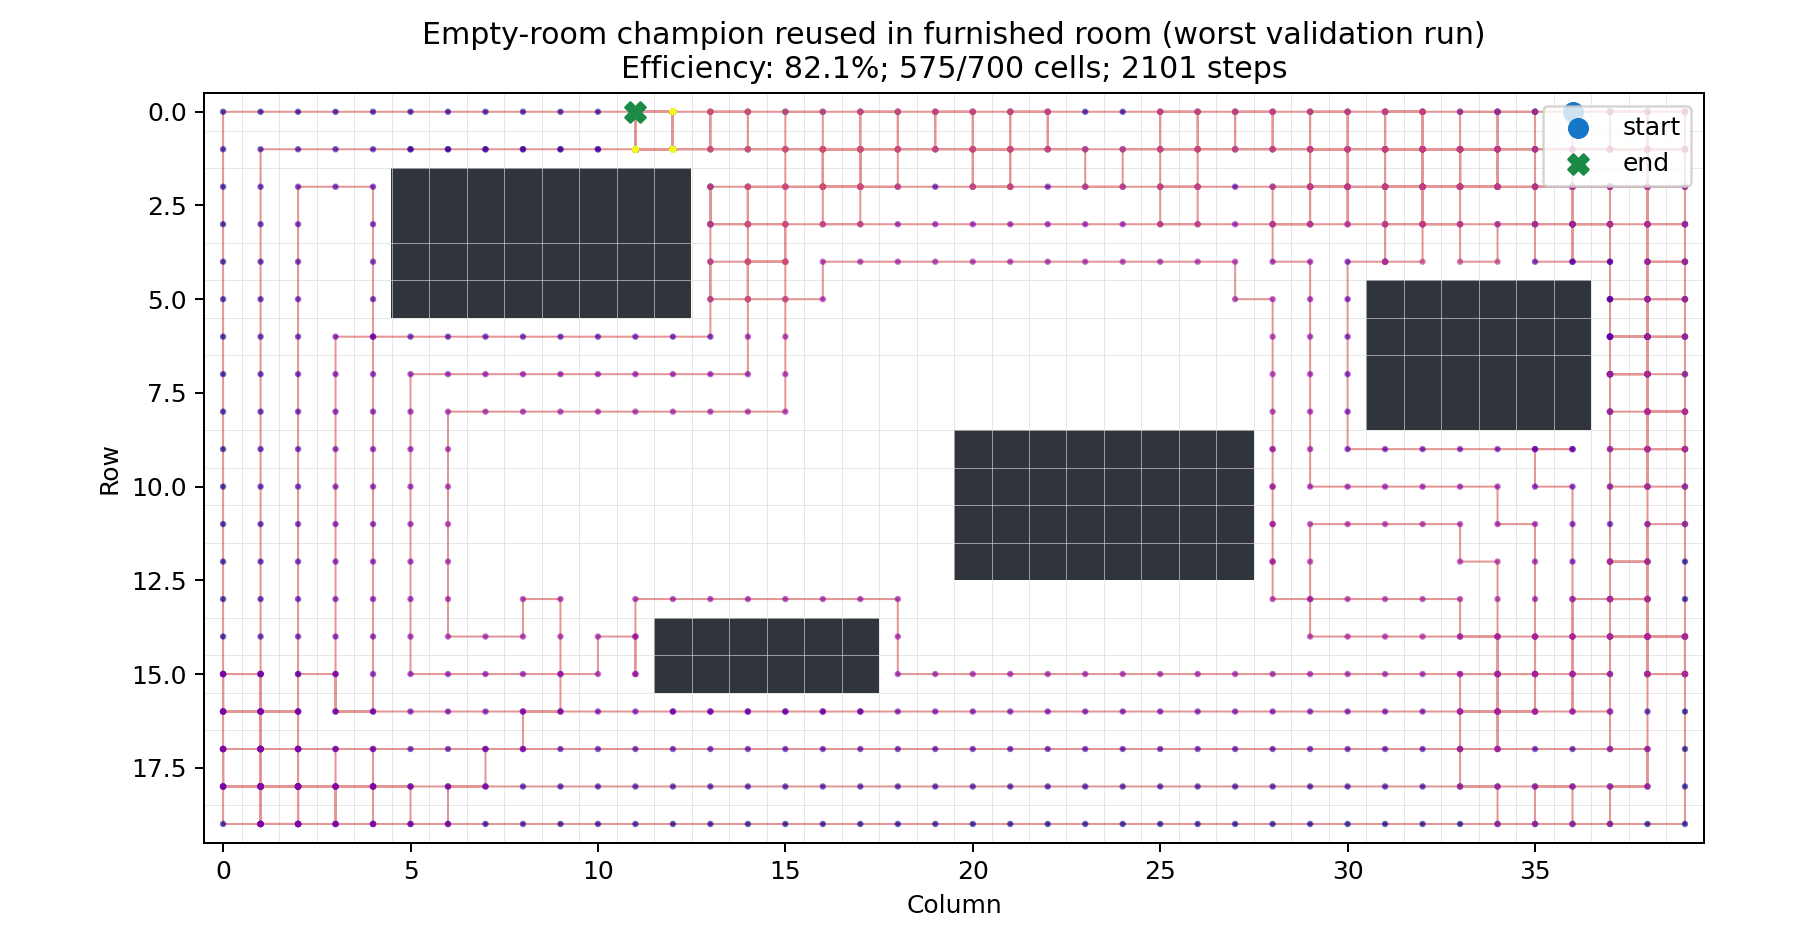
\includegraphics[width=0.46\textwidth]{outputs/furnished_reuse_worst_trajectory.png}
\caption{A successful transfer run and a lower-performing transfer run in the furnished room.}
\end{figure}

\begin{figure}[H]
\centering

\includegraphics[width=0.92\textwidth]{outputs/furnished_fitness.png}
\caption{Fitness over generations when the furnished room is used from the beginning.}
\end{figure}

\begin{figure}[H]
\centering

\includegraphics[width=0.92\textwidth]{outputs/furnished_best_trajectory.png}
\caption{Trajectory of the best chromosome evolved for the furnished room.}
\end{figure}

\section*{9. Conclusion}

The genetic algorithm discovers a useful local painter policy from only the four-cell state. In the empty room, the final champion covers nearly all floor space and reaches complete coverage on a validation start. However, the chromosome is specialized to the geometry seen during evolution. Furniture changes the local state distribution and breaks the learned sweep, making direct transfer less reliable. Evolving the same chromosome representation in the furnished environment recovers high and more consistent efficiency.

The Python implementation, plots, CSV fitness histories, and JSON summary are included in the deliverables folder. The executable source is included in the \texttt{code} folder.

\end{document}
